\documentclass[prb,11pt]{revtex4-1}

% preamble:

\usepackage{amsmath}    % need for subequations
\usepackage{graphicx}   % need for figures
\usepackage{verbatim}   % useful for program listings
\usepackage{color}      % use if color is used in text
\usepackage{subfigure}  % use for side-by-side figures
\usepackage{hyperref}   % use for hypertext links, including those to external documents and URLs
\raggedbottom           % don't add extra vertical space
\begin{comment}
\pagestyle{empty}       % use if page numbers not wanted
\end{comment}

\begin{document}

\title{Effective viscosity of polymer networks in the presence of cross-link slip}
\author{William McFadden}
\affiliation{University of Chicago, Biophysical Sciences Program, Chicago, IL 60615}

\date{1 January 2014}

\begin{abstract}
We are trying to describe the problem of what happens when cross-links relax stress in semi-flexible filament networks.  We have addressed the problem using a simplified model in which cross-links are allowed to slip past one another in a friction-like manner.  This model gives a prediction for the long timescale effective viscosity of the medium.  We have verified our solution using computational models of filaments in the limit where persistence length is much longer than filament length.  In this model, we find that network architectures and slip rates give rise to different modes of connectivity.
\end{abstract}

\maketitle

\section{Introduction}
Here, I talk about all the things that have ever happened of importance. And it goes on for a long time.
Lorem ipsum dolor sit amet, consectetur adipiscing elit, sed do eiusmod tempor incididunt ut labore et dolore magna aliqua. Ut enim ad minim veniam, quis nostrud exercitation ullamco laboris nisi ut aliquip ex ea commodo consequat. Duis aute irure dolor in reprehenderit in voluptate velit esse cillum dolore eu fugiat nulla pariatur. Excepteur sint occaecat cupidatat non proident, sunt in culpa qui officia deserunt mollit anim id est laborum.


\section{The Model}
Here I will include math and equations that explain what it is that I am talking about when I talk about a model.  It will involve writing the semi-flexible filament potential and then writing the coupling equation.  These are just placeholders for now, while I write these things out by hand first.
\begin{equation}
\Delta =\sum_{i=1}^N w_i (x_i - \bar{x})^2.
\end{equation}
It is a good idea to number equations, but we can have a
equation without a number:
\begin{equation}
P(x) = \frac{x - a}{b - a}, \nonumber
\end{equation}
and
\begin{equation}
g = \frac{1}{2} \sqrt{2\pi}. \nonumber
\end{equation}

We can give an equation a label so that we can refer to it later.
\begin{equation}
\label{eq:ising}
E = -J \sum_{i=1}^N s_i s_{i+1},
\end{equation}
Equation~\eqref{eq:ising} expresses the energy of a configuration
of spins in the Ising model.\footnote{REVTeX~4.1 places the footnotes in the bibliography. It is necessary to run BibTEX for footnotes to appear.}


\section{Analytical Results}
And this is where I prove by hand that some great amazing things can be seen about the system if we just take our little averages the right way.

\begin{equation}
I = \! \int_{-\infty}^\infty f(x)\,dx \label{eq:fine}.
\end{equation}
We can do some fine tuning by adding small amounts of horizontal
spacing:
\begin{verbatim}
 \, small space       \! negative space
\end{verbatim}
as is done in Eq.~\eqref{eq:fine}.



\section{Simulation Results}

We can make figures bigger or smaller by scaling them. Figure~\ref{fig:sine}
has been scaled by 60\%.

\begin{figure}[h!]
\centering
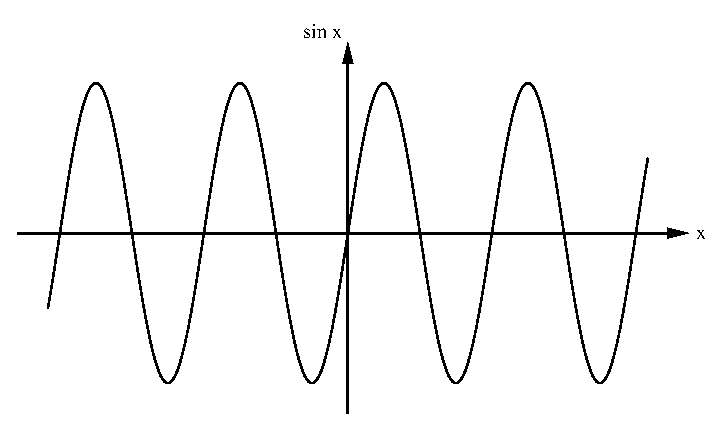
\includegraphics[scale=0.6]{sine}
\caption{\label{fig:sine}Show me a sine.}
\end{figure}

\section{Simulation details}
And I think I'll probably include all the gory details of how my simulations work since I'll be wanting to have direct references to the code. Use \verb+\begin{verbatim}+ and
\verb+\end{verbatim}+ as in the following example:
\begin{verbatim}
double y0 = 10; // example of declaration and assignment statement
double v0 = 0;  // initial velocity
double t = 0;   // time
double dt = 0.01; // time step
double y = y0;
\end{verbatim}
The command \verb+\verbatiminput{programs/Square.java}+ allows
you to list the file \texttt{Square.java} in the directory
programs.

\section{Discussion}

{\color{blue}{Finally I wax philosophical}},
{\color{green}{but}} {\color{cyan}{who is going pay for the ink?}}

\begin{thebibliography}{5}

\bibitem{latex}Helmut Kopka and Patrick W. Daly, \textsl{A Guide to
\LaTeX: Document Preparation for Beginners and Advanced Users} (Addison-Wesley, 2004), 4th ed.

\bibitem{website}Some useful links are
given at \url{<sip.clarku.edu/tutorials/TeX/>}.

\end{thebibliography}

\end{document}